\chapter{الطفرات والتنوع الوراثي}\label{ch:g11:mutations}

يولد طفل بلا صباغ البتة --- شعر أبيض، وجلد شاحب، وعينان لا تحتملان
الضوء الساطع --- لوالدين عاديين من عائلة لا تاريخ لها بهذه الحال.
ومستعمرة بكتيريا لم تلق مضادًا حيويًا قط تحوي، من بين مئة مليون \omterm{def:g10:cells-common-unit:cell}{خلية}،
قليلًا يقاومه من قبل. ويجد بستاني غصنًا واحدًا في شجيرة ورد يحمل
أزهارًا بلون آخر. في كل حالة تغيرت متتالية من \omterm{def:g10:universal-dna:information}{DNA}، مرة واحدة، في \omterm{def:g10:cells-common-unit:cell}{خلية}
واحدة؛ وفي كل حالة ينسخ التغير بأمانة بعد ذلك. وهذا الفصل عن تلك
التغيرات: ما هي، ومن أين تأتي، وكيف تحد \omterm{def:g10:cells-common-unit:cell}{الخلية} منها، ولماذا تتوقف
الحياة على ألا تتوقف هي أبدًا تمامًا.

\section{ما الطفرة}

\begin{definition}[الطفرة]\label{def:g11:mutations:mutation}
\emph{الطفرة}\index{طفرة} تغير في متتالية نوكليوتيدات جزيء \omterm{def:g10:universal-dna:information}{DNA}، ينتقل
إلى ذرية \omterm{def:g10:cells-common-unit:cell}{الخلية} التي وقع فيها. وأشيعها \emph{الطفرات النقطية}، وهي
تصيب نوكليوتيدًا واحدًا أو بضعة:
\begin{itemize}
  \item \emph{الاستبدال}: \omterm{def:g10:universal-dna:nucleotide}{نوكليوتيد} يحل محله آخر؛
  \item \emph{الإقحام}: \omterm{def:g10:universal-dna:nucleotide}{نوكليوتيد} أو أكثر يضاف؛
  \item \emph{الحذف}: \omterm{def:g10:universal-dna:nucleotide}{نوكليوتيد} أو أكثر يزال.
\end{itemize}
والتغيرات الأكبر --- قطعة تضاعف أو تنقلب أو تنقل، أو \omterm{def:g10:universal-dna:information}{صبغي} كامل يكتسب
أو يفقد --- طفرات كذلك.
\end{definition}

\begin{omfigure}
\begin{tikzpicture}[font=\small\ttfamily]
  \tikzset{seq/.style={anchor=west}}
  \node[seq] at (0,0) {\textrm{الأصل}\ \ \ \ \ \ \ ATG GCT TAC GGA TCC};
  \node[seq] at (0,-0.8) {\textrm{استبدال}\ \ \ \ \ ATG GCT T\textcolor{omThm}{\textbf{G}}C GGA TCC};
  \node[seq] at (0,-1.6) {\textrm{إقحام}\ \ \ \ \ \ \ ATG GCT TA\textcolor{omThm}{\textbf{A}} CGG ATC C};
  \node[seq] at (0,-2.4) {\textrm{حذف}\ \ \ \ \ \ \ \ ATG GCT T\textcolor{omThm}{\textbf{\_}}C GGA TCC};
  \node[seq, font=\small] at (7.9,-0.8) {حرف واحد تغير};
  \node[seq, font=\small] at (7.9,-1.6) {حرف واحد أضيف: فانزاح كل ما يليه};
  \node[seq, font=\small] at (7.9,-2.4) {حرف واحد أزيل: فانزاح كل ما يليه};
\end{tikzpicture}

{\small ثلاث \omterm{def:g11:mutations:mutation}{طفرات} نقطية للمتتالية نفسها (والأحرف مجمّعة ثلاثًا ثلاثًا
لسبب يفسره \cref{ch:g11:gene-expression}). فالاستبدال يغير موضعًا
واحدًا؛ أما الإقحام أو الحذف فيزيح كل ما بعده.}
\end{omfigure}

\begin{proposition}[أين تقع الطفرات، وعند من]\label{prop:g11:mutations:where}
\omterm{def:g11:mutations:mutation}{الطفرة} التي تقع في \omterm{def:g10:cells-common-unit:cell}{خلية} جسدية (\emph{\omterm{def:g11:mutations:mutation}{طفرة} جسدية}) تنتقل إلى ذرية تلك
\omterm{def:g10:cells-common-unit:cell}{الخلية} وحدها: أي إلى رقعة من نسيج على الأكثر، في فرد واحد. أما \omterm{def:g11:mutations:mutation}{الطفرة}
في \omterm{def:g10:cells-common-unit:cell}{خلية} جنسية --- مشيج أو أحد سلائفه --- فتنتقل إلى النسل الذي يحبل
منه وإلى كل \omterm{def:g10:cells-common-unit:cell}{خلية} من خلاياه: و\emph{\omterm{def:g11:mutations:mutation}{الطفرة} السلالية} هي الصنف الوحيد
الذي يدخل في وراثة \omterm{def:g10:biodiversity-scales:species}{النوع}. فغصن شجيرة الورد الغريب \omterm{def:g11:mutations:mutation}{طفرة} جسدية؛ أما حال
الطفل عديم الصباغ فجاءت من \omterm{def:g11:mutations:mutation}{طفرة} سلالية عند سلف ما، حملت صامتة أجيالًا.
\end{proposition}
\admitted

\begin{example}[تواتر الطفرات]\label{ex:g11:mutations:frequency}
يخلّف التضاعف نحو خطأ واحد لكل $10^9$ \omterm{def:g10:universal-dna:nucleotide}{نوكليوتيد}
(\cref{ch:g11:dna-replication}). \omterm{def:g10:universal-dna:gene}{فمورّثة} فيها $\num{3000}$ زوج قواعد
ينسخ فيها إذن خطأ نحو مرة في كل $\num{300000}$ تضاعف؛ والإنسان، وينسخ
مجينه نحو $10^{16}$ مرة في العمر، تتراكم عنده \omterm{def:g11:mutations:mutation}{طفرات} في كل \omterm{def:g10:universal-dna:gene}{مورّثة} في
\omterm{def:g10:cells-common-unit:cell}{خلايا} كثيرة. ويولد كل طفل بنحو 60 \omterm{def:g11:mutations:mutation}{طفرة} جديدة لم يحملها أي من والديه
--- وكلها تقريبًا في 98\% من المجين التي ليست \omterm{def:g10:universal-dna:gene}{مورّثات}.
\end{example}

\section{الأسباب: عفوية ومستحثة}

\begin{proposition}[الطفرات العفوية]\label{prop:g11:mutations:spontaneous}
تنشأ \omterm{def:g11:mutations:mutation}{الطفرات} في كل \omterm{def:g10:cells-common-unit:cell}{خلية}، من دون أي عامل خارجي: من الازدواجات الخاطئة
النادرة التي تفلت من تحقق البوليميراز، ومن عدم استقرار \omterm{def:g10:universal-dna:information}{DNA} الكيميائي
نفسه، إذ تتضرر قواعده آلاف المرات في اليوم في كل \omterm{def:g10:cells-common-unit:cell}{خلية} بالماء وبجزيئات
\omterm{def:g10:cell-metabolism:metabolism}{الاستقلاب} العادي الفعالة. وهذه \emph{\omterm{def:g11:mutations:mutation}{الطفرات} العفوية}
\emph{عشوائية}: فهي تقع في أي موضع، بنسبة لا تتوقف على ما إذا كان
التغير سينفع \omterm{def:g10:cells-common-unit:cell}{الخلية}.
\end{proposition}
\begin{proof}[شواهد]
نثر ليدربرغ (1952) بكتيريا لم تعرض قط لمضاد حيوي على طبق، وتركها تنمو
مستعمرات، ثم ضغط وسادة من المخمل على الطبق وطبع بصمتها --- المستعمرات
نفسها في المواضع نفسها --- على عدة أطباق تحوي المضاد الحيوي. فظهرت
المستعمرات المقاومة القليلة في \emph{المواضع نفسها} على كل طبق مضاد.
ولما كانت آتية من مستعمرات الطبق الأصلي نفسها، وهو لم ير المضاد قط،
كانت \omterm{def:g11:mutations:mutation}{طفرة} المقاومة موجودة قبل التعرض: فالمضاد كشفها ولم يسببها. وقد
وقعت \omterm{def:g11:mutations:mutation}{الطفرات} عشوائيًا أثناء نمو المستعمرات، بلا نظر إلى نفعها المقبل.
\end{proof}

\begin{omfigure}
\begin{tikzpicture}[font=\small, >=Stealth]
  \tikzset{plate/.style={draw, thick, circle, minimum size=2.4cm, fill=omDef!6}}
  \node[plate] (p0) at (0,0) {};
  \foreach \x/\y in {-0.6/0.5, 0.3/0.7, -0.2/-0.2, 0.7/-0.1, -0.7/-0.6, 0.4/-0.7, 0.0/0.25, -0.35/0.85}
    \fill[omDef!60] (\x,\y) circle (2.2pt);
  \fill[omThm] (0.3,0.7) circle (2.6pt); \fill[omThm] (-0.7,-0.6) circle (2.6pt);
  \node[anchor=north, align=center] at (0,-1.35) {الطبق الأصلي،\\ بلا مضاد حيوي};
  \node[draw, fill=gray!25, minimum width=2.4cm, minimum height=0.35cm] (v) at (3.6,0) {مخمل};
  \draw[->, thick] (1.3,0) -- (v.west);
  \node[plate, fill=omProp!8] (p1) at (7.0,1.5) {};
  \node[plate, fill=omProp!8] (p2) at (7.0,-1.5) {};
  \draw[->, thick] (v.east) -- (5.7,1.2);
  \draw[->, thick] (v.east) -- (5.7,-1.2);
  \fill[omThm] (7.3,2.2) circle (2.6pt); \fill[omThm] (6.3,0.9) circle (2.6pt);
  \fill[omThm] (7.3,-0.8) circle (2.6pt); \fill[omThm] (6.3,-2.1) circle (2.6pt);
  \node[anchor=west, align=left] at (8.3,1.5) {طبق بمضاد حيوي:\\ الموضعان نفسهما};
  \node[anchor=west, align=left] at (8.3,-1.5) {طبق بمضاد حيوي:\\ الموضعان نفسهما};
\end{tikzpicture}

{\small الطبع بالنسخ. المستعمرات التي نمت بلا مضاد حيوي تطبع على أطباق
بمضاد. فتظهر المستعمرات المقاومة (بالأحمر) في مواضع متطابقة على كل
نسخة: فالمقاومة كانت موجودة في المستعمرات الأصلية، قبل أي تماس مع
الدواء.}
\end{omfigure}

\begin{definition}[المطفِّر]\label{def:g11:mutations:mutagen}
\emph{المطفِّر}\index{مطفر} عامل فيزيائي أو كيميائي يرفع نسبة \omterm{def:g11:mutations:mutation}{الطفرات}
بإضراره بجزيء \omterm{def:g10:universal-dna:information}{DNA}. فالضوء فوق البنفسجي يلحم تيمينين متجاورين على شريط؛
والأشعة السينية والنشاط الإشعاعي تقطع الشرائط؛ والمواد الكيميائية مثل
بنزوبيرين دخان التبغ أو أفلاتوكسين الحبوب المعفنة تلتصق بالقواعد وتشوه
اللولب. \omterm{def:g10:cells-common-unit:cell}{والخلية} التي تتعرض لمطفِّر تحمل \emph{\omterm{def:g11:mutations:mutation}{طفرات} مستحثة} إلى جانب
طفراتها العفوية --- وهي أيضًا في مواضع عشوائية، لكنها أكثر عددًا.
\end{definition}

\begin{example}[فوق البنفسجي على الخميرة]\label{ex:g11:mutations:uv}
\omterm{def:g10:cells-common-unit:cell}{خلايا} خميرة تنثر على أطباق وتعرض للضوء فوق البنفسجي مددًا متزايدة:
فبعد \qty{10}{s} يخفق نصف \omterm{def:g10:cells-common-unit:cell}{الخلايا} في تكوين مستعمرة، وبعد \qty{20}{s}
ربعها، وبعد \qty{30}{s} ثمنها --- فكل جرعة تنصّف الناجيات. وبين
الناجيات، ترتفع نسبة المستعمرات ذوات الصفة المتغيرة تغيرًا مرئيًا
(لونًا أو شكلًا أو عجزًا عن النمو على سكر معين) من واحدة في المليون
إلى واحدة في الألف. فالمصباح يقتل بإضراره بجزيء \omterm{def:g10:universal-dna:information}{DNA} ضررًا لا يصلح، ويطفّر
بإضراره به دون ذلك بقليل.
\end{example}

\begin{omfigure}
\begin{tikzpicture}
\begin{axis}[
  width=0.86\linewidth, height=5.6cm,
  axis x line=bottom, axis y line=left,
  xmin=0, xmax=65, ymin=0, ymax=110,
  xlabel={التعرض لفوق البنفسجي (s)}, ylabel={الناجيات (\%)},
  xlabel style={font=\small, at={(axis description cs:0.5,-0.12)}, anchor=north},
  ylabel style={font=\small},
  tick label style={font=\small}, xtick={0,10,20,30,40,50,60}, ytick={0,25,50,75,100},
  legend style={at={(0.97,0.95)}, anchor=north east, font=\small, draw=none},
  legend cell align=left,
]
\addplot[thick, omDef, mark=*, mark size=1.5pt] coordinates
  {(0,100) (10,50) (20,25) (30,12.5) (40,6.3) (50,3.1) (60,1.6)};
\addplot[thick, omThm, dashed, mark=square*, mark size=1.5pt] coordinates
  {(0,100) (10,10) (20,1) (30,0.1) (40,0.01)};
\legend{{خميرة عادية}, {خميرة تنقصها إنزيمة إصلاح}}
\end{axis}
\end{tikzpicture}

{\small بقاء \omterm{def:g10:cells-common-unit:cell}{خلايا} الخميرة بدلالة التعرض لفوق البنفسجي. \omterm{def:g10:cells-common-unit:cell}{الخلايا}
العادية تفقد نصف عددها كل \qty{10}{s}؛ وسلالة عاجزة عن إصلاح ضرر فوق
البنفسجي تفقد تسعة أعشارها كل \qty{10}{s}. والفرق هو عمل الإصلاح.}
\end{omfigure}

\begin{omfigure}
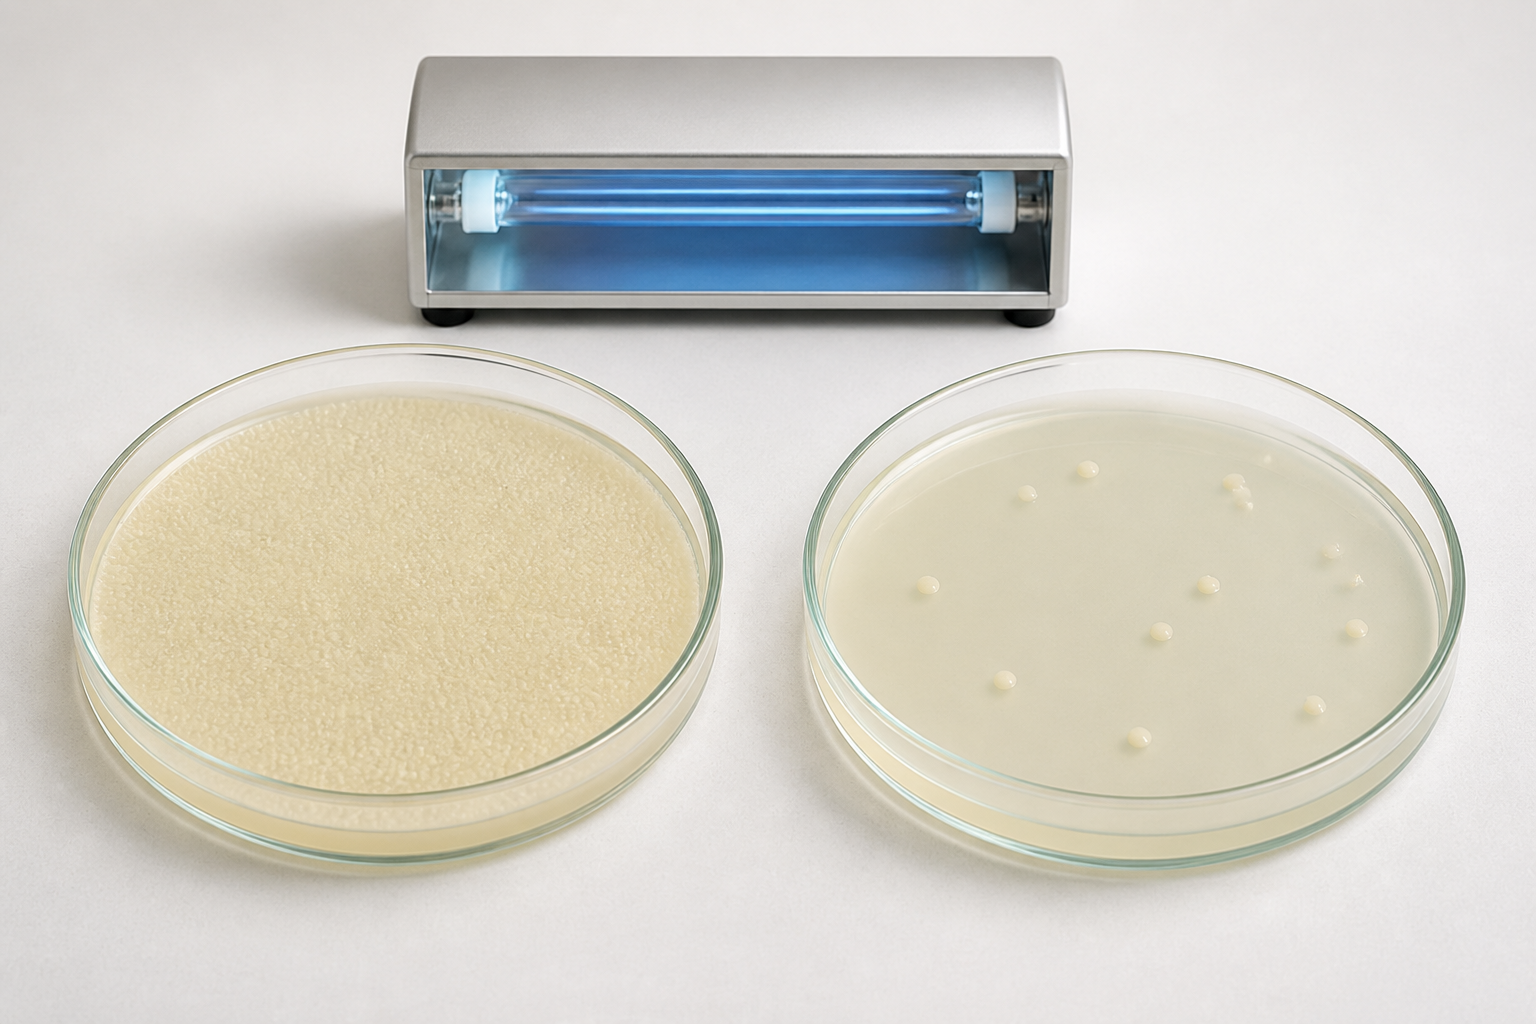
\includegraphics[width=0.6\linewidth]{images/book2/ai/g11-mutation-uv-plates.png}

{\small طبقان بذرت فيهما البكتيريا نفسها. اليسار: بلا تعريض، مرج متصل.
واليمين: بعد التعريض لفوق البنفسجي، لم ينم مستعمرات إلا \omterm{def:g10:cells-common-unit:cell}{الخلايا} التي
أصلح ضرر \omterm{def:g10:universal-dna:information}{DNA} فيها في الوقت المناسب.}
\end{omfigure}

\section{الخلية تدافع: الإصلاح}

\begin{proposition}[إصلاح DNA]\label{prop:g11:mutations:repair}
تصاب \omterm{def:g10:cells-common-unit:cell}{الخلية} بعشرات الألوف من آفات \omterm{def:g10:universal-dna:information}{DNA} في اليوم ولا تكاد تحتفظ بشيء
منها: فأنظمة إنزيمية مخصصة تجوب \omterm{prop:g10:universal-dna:helix}{اللولب المزدوج}، وتتعرف قاعدة متضررة أو
مزدوجة خطأً، وتقطع القطعة المعيبة من أحد الشريطين وتعيد بناءها
بالشريط الآخر أصلًا --- أي تتام \cref{ch:g10:universal-dna} من جديد.
ولا تصير الآفة \omterm{def:g11:mutations:mutation}{طفرة} إلا إذا أفلتت من الإصلاح قبل أن ينسخها التضاعف
التالي. والإصلاح هو سبب كون نسبة \omterm{def:g11:mutations:mutation}{الطفرات} $10^{-9}$ لا $10^{-5}$.
\end{proposition}
\begin{proof}[شواهد]
المصابون بالحالة الوراثية جفاف الجلد المصطبغ تنقصهم إنزيمة من
الإنزيمات التي تستأصل ضرر فوق البنفسجي. فجلودهم، إذا تعرضت لضوء النهار
العادي، تصاب بالسرطانات ألف مرة أكثر من الجلد الطبيعي ومنذ الطفولة
الباكرة؛ وإذا حميت من الشمس كانت طبيعية. فوق البنفسجي نفسه، والآفات
نفسها --- لكن من دون الإصلاح تبقى الآفات، وتتراكم \omterm{def:g11:mutations:mutation}{الطفرات} في
\omterm{def:g10:universal-dna:gene}{المورّثات} التي تضبط انقسام \omterm{def:g10:cells-common-unit:cell}{الخلية} (\cref{ch:g11:cancer}). وسلالات
الخميرة والبكتيريا التي تنقصها إنزيمات الإصلاح تبين فرط الحساسية نفسه
في المختبر.
\end{proof}

\begin{omfigure}
\begin{tikzpicture}[font=\small, >=Stealth,
  b/.style={draw, rounded corners, align=center, text width=2.6cm, minimum height=1.1cm}]
  \node[b, fill=omProp!15] (a) at (0,0) {فوق البنفسجي يلحم\\ حرفي T متجاورين};
  \node[b, fill=omDef!12] (bx) at (3.4,0) {إنزيمات الإصلاح\\ تكشف التشوه};
  \node[b, fill=omDef!12] (c) at (6.8,0) {القطعة المتضررة\\ تقطع من شريط};
  \node[b, fill=omDef!12] (d) at (10.2,0) {الفجوة تملأ بالاعتماد\\ على الشريط السليم};
  \draw[->] (a) -- (bx); \draw[->] (bx) -- (c); \draw[->] (c) -- (d);
  \node[b, fill=omThm!12] (e) at (3.4,-2.0) {التضاعف ينسخ\\ الآفة};
  \node[b, fill=omThm!12] (f) at (6.8,-2.0) {طفرة، صارت\\ دائمة};
  \draw[->] (a.south) |- node[pos=0.25, left, font=\scriptsize, align=right] {إن لم تصلح\\ في الوقت} (e.west);
  \draw[->] (e) -- (f);
\end{tikzpicture}

{\small السباق بين الإصلاح والتضاعف. الآفة التي تستأصل ويعاد بناؤها من
الشريط الآخر لا تخلف أثرًا؛ أما الآفة التي لا تزال موجودة حين تمر
الشوكة فتنسخ في المتتالية وتصير \omterm{def:g11:mutations:mutation}{طفرة}.}
\end{omfigure}

\section{عواقب الطفرة}

\begin{proposition}[من المتتالية إلى النمط الظاهري]\label{prop:g11:mutations:consequences}
\omterm{def:g11:mutations:mutation}{الطفرة} تحوّل أليلًا إلى \omterm{def:g10:universal-dna:gene}{أليل} جديد. ويتوقف أثرها على موضع وقوعها وعلى
ما تفعله \omterm{def:g10:chemistry-of-life:families}{بالبروتين} الذي ترمز له \omterm{def:g10:universal-dna:gene}{المورّثة}
(و\cref{ch:g11:gene-expression} يعطي القواعد):
\begin{itemize}
  \item خارج أي \omterm{def:g10:universal-dna:gene}{مورّثة}، أو في موضع لا يغير \omterm{def:g10:chemistry-of-life:families}{البروتين}: \emph{لا أثر}
        --- وهي الأغلبية الساحقة؛
  \item داخل \omterm{def:g10:universal-dna:gene}{مورّثة}، وتغير حمضًا أمينيًا واحدًا: \omterm{def:g10:chemistry-of-life:families}{بروتين} يعمل بصورة
        مختلفة قليلًا، أو لا يعمل البتة، أو يعمل أحيانًا على نحو
        أفضل؛
  \item داخل \omterm{def:g10:universal-dna:gene}{مورّثة}، وتزيح الرسالة أو تبترها: \omterm{def:g10:chemistry-of-life:families}{بروتين} لا يعمل عادةً.
\end{itemize}
وأما كون \omterm{def:g10:chemistry-of-life:families}{البروتين} المتغير ضارًا أو محايدًا أو نافعًا فيتوقف على
المحيط: \omterm{def:g10:universal-dna:gene}{فالأليل} نفسه \omterm{def:g10:universal-dna:gene}{لمورّثة} الهيموغلوبين عبء في منطقة بلا ملاريا
وحماية حيث توجد الملاريا.
\end{proposition}
\admitted

\begin{example}[صباغ فُقد، وصباغ حُفظ]\label{ex:g11:mutations:pigment}
صباغ الميلانين يصنعه \omterm{def:g10:cell-metabolism:metabolism}{إنزيم}. وتعرف عشرات \omterm{def:g11:mutations:mutation}{الطفرات} المختلفة لمورّثته،
تنتج كل منها إنزيمًا لا يعمل، وتنتج عند شخص يحمل \omterm{def:g10:universal-dna:gene}{أليلين} من هذا القبيل
حالَ انعدام الصباغ التي افتتح بها الفصل. وقد نشأ كل منها عشوائيًا،
مرة واحدة، في \omterm{def:g10:cells-common-unit:cell}{خلية} جنسية؛ ولا تظهر الحال المرئية إلا حين يورث حاملان
أليليهما الصامتين الطفل نفسه. \omterm{def:g10:universal-dna:gene}{والمورّثة} نفسها، في \omterm{def:g10:universal-dna:gene}{أليل} آخر، تصنع
إنزيمًا أقل نشاطًا قليلًا --- ومنه جلد أفتح، وهو شائع في جمهرات عاشت
آلاف السنين في خطوط عرض عالية، حيث يتيح صباغ أقل قليلًا للجلد أن يصنع
فيتامين D أكثر من شمس ضعيفة.
\end{example}

\begin{proposition}[الطفرة، مصدر التنوع]\label{prop:g11:mutations:source}
كل \omterm{def:g10:universal-dna:gene}{أليل} لكل \omterm{def:g10:universal-dna:gene}{مورّثة} بدأ طفرةً \omterm{def:g10:universal-dna:gene}{لأليل} أسبق. \omterm{def:g11:mutations:mutation}{والطفرة} هي العملية الوحيدة
التي تخلق \omterm{def:g10:universal-dna:information}{معلومة وراثية} جديدة؛ أما الخلط الجنسي في السنة الأخيرة فلا
يفعل إلا أن يعيد تركيب ما صنعته \omterm{def:g11:mutations:mutation}{الطفرة}. \omterm{def:g11:mutations:mutation}{والطفرة}، على ندرتها وعشوائيتها
وكونها محايدة أو ضارة في الفرد غالبًا، هي مع ذلك ما يوفر، عبر الأجيال،
التنوع الذي يتوقف عليه تطور \cref{ch:g10:biodiversity-scales}.
\end{proposition}
\admitted

\begin{method}[تحليل طفرة]\label{met:g11:mutations:analyse}
\begin{enumerate}
  \item قارن المتتالية الطافرة بالأصلية، حرفًا حرفًا، وسمِّ التغير
        (استبدال، أو إقحام، أو حذف؛ وكم نوكليوتيدًا).
  \item عيّن موضعها: في \omterm{def:g10:universal-dna:gene}{مورّثة} أم خارجها؛ وإن كانت في \omterm{def:g10:universal-dna:gene}{مورّثة}، فهل
        انزاحت قراءة الرسالة.
  \item عيّن \omterm{def:g10:cells-common-unit:cell}{الخلية} التي وقعت فيها: جسدية (فرد واحد، نسيج واحد) أم
        سلالية (منقولة).
  \item ابحث عن سبب إن كانت النسبة غير معتادة (تعرض لمطفِّر، أو إصلاح
        معيب)؛ وإلا فانسبها إلى المصادفة.
  \item احكم على العاقبة على مستوى \omterm{def:g10:chemistry-of-life:families}{البروتين}، ثم \omterm{def:g10:cells-common-unit:cell}{الخلية}، ثم الكائن، ثم
        الجمهرة --- بهذا الترتيب، وفي محيط مذكور.
\end{enumerate}
\end{method}

\begin{remark}[العشوائية، بدقة]\label{rem:g11:mutations:random}
«عشوائية» لا تعني أن كل المواضع تطفر بالقدر نفسه --- فبعض المتتاليات
أهش --- ولا أن \omterm{def:g11:mutations:mutation}{الطفرات} بلا سبب. إنما تعني أن وقوع \omterm{def:g11:mutations:mutation}{الطفرة} مستقل عما إذا
كانت ستنفع \omterm{def:g10:cells-common-unit:cell}{الخلية}: فالبكتيريا المقاومة للمضاد الحيوي في أطباق النسخ لم
يجعلها المضاد مقاومة، وما من كائن يستطيع أن «يقرر» أن يطفر في اتجاه
نافع. والانتقاء هو الذي يوجّه، بعد ذلك؛ أما \omterm{def:g11:mutations:mutation}{الطفرة} فلا تفعل إلا أن
توفر.
\end{remark}

\section{تمارين}

\begin{exercise}[$\star$]\label{exo:g11:mutations:1}
عرّف \omterm{def:g11:mutations:mutation}{الطفرة} وسمِّ أصناف \omterm{def:g11:mutations:mutation}{الطفرة} النقطية الثلاثة.
\end{exercise}

\begin{exercise}[$\star$]\label{exo:g11:mutations:2}
قارن \texttt{ATGCCTGAAT} بالطافرات \texttt{ATGCCAGAAT}
و\texttt{ATGCCTGAT} و\texttt{ATGCCTTGAAT}. سمِّ كل \omterm{def:g11:mutations:mutation}{طفرة}.
\end{exercise}

\begin{exercise}[$\star$]\label{exo:g11:mutations:3}
ما الفرق بين \omterm{def:g11:mutations:mutation}{الطفرة} الجسدية \omterm{def:g11:mutations:mutation}{والطفرة} السلالية؟ وأيهما يهم الوراثة؟
\end{exercise}

\begin{exercise}[$\star$]\label{exo:g11:mutations:4}
سمِّ ثلاثة مطفِّرات، وأعطِ لأحدها الضرر الذي يلحقه بجزيء \omterm{def:g10:universal-dna:information}{DNA}.
\end{exercise}

\begin{exercise}[$\star$]\label{exo:g11:mutations:5}
ما الذي يستعمله نظام الإصلاح أصلًا ليعيد بناء قطعة متضررة؟ ولماذا كان
ذلك ممكنًا؟
\end{exercise}

\begin{exercise}[$\star\star$]\label{exo:g11:mutations:6}
من شكل البقاء، أي نسبة من الخميرة العادية تنجو من \qty{40}{s} من فوق
البنفسجي؟ وأي نسبة من السلالة الناقصة الإصلاح؟ وبأي عامل يحسّن الإصلاح
البقاء عند تلك الجرعة؟
\end{exercise}

\begin{exercise}[$\star\star$]\label{exo:g11:mutations:7}
مزرعة من $10^9$ بكتيريا تنثر على طبق بمضاد حيوي فتنمو 20 مستعمرة.
قدّر تواتر \omterm{def:g10:cells-common-unit:cell}{الخلايا} المقاومة. وهل يخبرك ذلك بأن المضاد الحيوي هو الذي
سبب \omterm{def:g11:mutations:mutation}{الطفرة}؟
\end{exercise}

\begin{exercise}[$\star\star$]\label{exo:g11:mutations:8}
فسّر بكلماتك لماذا تثبت المواضع المتطابقة للمستعمرات المقاومة على
أطباق النسخ أن \omterm{def:g11:mutations:mutation}{الطفرات} وقعت قبل التعرض.
\end{exercise}

\begin{exercise}[$\star\star$]\label{exo:g11:mutations:9}
\omterm{def:g10:universal-dna:gene}{مورّثة} فيها \num{3000} زوج قواعد تنسخ بخطأ واحد لكل $10^9$ \omterm{def:g10:universal-dna:nucleotide}{نوكليوتيد}.
ففي نسيج من $10^{12}$ \omterm{def:g10:cells-common-unit:cell}{خلية}، كلها منحدرة من \omterm{def:g10:cells-common-unit:cell}{خلية} واحدة بأربعين انقسامًا،
كم \omterm{def:g10:cells-common-unit:cell}{خلية} تحمل تقريبًا \omterm{def:g11:mutations:mutation}{طفرة} جديدة في تلك \omterm{def:g10:universal-dna:gene}{المورّثة}؟ (لا تعد إلا الأخطاء
المرتكبة في الانقسام الأخير.)
\end{exercise}

\begin{exercise}[$\star\star$]\label{exo:g11:mutations:10}
شجيرة ورد تحمل غصنًا واحدًا بأزهار من لون آخر. والعقل المأخوذة من ذلك
الغصن تعطي شجيرات باللون الجديد؛ أما بذور أزهاره فتعطي ورودًا عادية.
فسّر النتيجتين.
\end{exercise}

\begin{exercise}[$\star\star$]\label{exo:g11:mutations:11}
لماذا يصاب المصاب بجفاف الجلد المصطبغ بسرطانات الجلد ولا يصاب، مثلًا،
بسرطانات المعي؟
\end{exercise}

\begin{exercise}[$\star\star\star$]\label{exo:g11:mutations:12}
واقي الشمس يمتص فوق البنفسجي. باستعمال شكل البقاء، فسّر ما الذي يفعله
واقٍ يمرر عشر فوق البنفسجي بعدد الآفات في \omterm{def:g10:cells-common-unit:cell}{خلية} الجلد في ساعة من الشمس،
ولماذا لا يعني «لا حروق شمس» «لا \omterm{def:g11:mutations:mutation}{طفرات}».
\end{exercise}

\begin{exercise}[$\star\star\star$]\label{exo:g11:mutations:13}
\omterm{def:g10:universal-dna:gene}{أليل} \omterm{def:g10:universal-dna:gene}{لمورّثة} الهيموغلوبين يحمي من الملاريا عند حاملي نسخة واحدة لكنه
يسبب مرضًا شديدًا عند حاملي نسختين. ناقش ما إذا كانت هذه \omterm{def:g11:mutations:mutation}{الطفرة} «ضارة»
أم «نافعة»، وما الذي يقرر ذلك.
\end{exercise}

\begin{exercise}[$\star\star\star$]\label{exo:g11:mutations:14}
بكتيريا في مرق بلا مضاد حيوي توجد فيها، بعد 30 جيلًا، \omterm{def:g10:cells-common-unit:cell}{خلية} مقاومة
واحدة لكل مليون. فإذا أضيف المضاد عندئذ، فماذا يحدث للمزرعة في غضون
يوم؟ فسّر لماذا يصر الأطباء على أخذ جرعة المضاد الحيوي كاملة.
\end{exercise}

\begin{exercise}[$\star\star\star$]\label{exo:g11:mutations:15}
«إذا كانت \omterm{def:g11:mutations:mutation}{الطفرات} ضارة دائمًا تقريبًا، فلا يمكن بناء التطور عليها.»
ناقش في فقرة، مستعملًا مفاهيم العشوائية، ونسبة \omterm{def:g11:mutations:mutation}{الطفرات} المحايدة،
والمحيط، وسلّم الزمن.
\end{exercise}

\section{مسألة: ختم المخمل}

\begin{problem}[{مسألة نهاية الأسبوع --- إعادة بناء الطبع بالنسخ عند
ليدربرغ: مستعمرات تعد، ومقاومات ترسم خرائطها، وأصل الطفرات يحسم،
ونسبتها تقاس}]
\label{pb:g11:mutations:1}
ينثر تلميذ نحو 200 بكتيريا، من مزرعة لم تلق المضاد الحيوي
الستربتوميسين قط، على طبق بلا مضاد. وبعد ليلة، نمت 200 مستعمرة، كل
منها من \omterm{def:g10:cells-common-unit:cell}{خلية} واحدة وكل منها تحوي نحو $10^7$ \omterm{def:g10:cells-common-unit:cell}{خلية}. ثم تضغط وسادة مخمل
على الطبق وتطبع على ثلاثة أطباق تحوي الستربتوميسين. وفي اليوم التالي،
يبين الطبق A مستعمرتين مقاومتين، والطبق B مستعمرتين، والطبق C
مستعمرتين --- في الموضعين نفسيهما على الأطباق الثلاثة.

\medskip
\noindent\textbf{الجزء الأول --- التجربة.}
\begin{enumerate}
  \item لماذا يجب أن تأتي مستعمرات الطبق الأصلي من \omterm{def:g10:cells-common-unit:cell}{خلايا} مفردة، ولماذا
        يبقى عدد البكتيريا المنثورة صغيرًا؟
  \item فسّر ما الذي ينقله المخمل، ولماذا يحفظ موضع المستعمرة.
  \item موضعان من أصل 200 يعطيان مستعمرات مقاومة على كل نسخة. فما الذي
        يبينه اتفاق النسخ الثلاث؟
  \item افترض بدلًا من ذلك أن المضاد الحيوي يستحث المقاومة في نسبة
        صغيرة من \omterm{def:g10:cells-common-unit:cell}{الخلايا} عند التماس. صف النمط الذي كانت النسخ الثلاث
        لتبينه عندئذ.
  \item أي الفرضيتين --- \omterm{def:g11:mutations:mutation}{طفرة} قبل التماس، أم استحثاث بالتماس ---
        يدعمها النمط المشاهد؟ اذكر الحجة في جملة واحدة.
\end{enumerate}

\medskip
\noindent\textbf{الجزء الثاني --- رجوعًا إلى الطبق الأصلي.}
\begin{enumerate}[resume]
  \item يأخذ التلميذ \omterm{def:g10:cells-common-unit:cell}{خلايا} من الموضعين المقاومين على الطبق
        \emph{الأصلي} (وهو لم يمس المضاد قط) ومن موضعين آخرين، ويختبر
        كل عينة على الستربتوميسين. تنبأ بالنتائج.
  \item المستعمرتان في الموضعين المقاومين تحوي كل منهما نحو $10^7$
        \omterm{def:g10:cells-common-unit:cell}{خلية}. فهل كل خلاياهما مقاومة أم بعضها فقط؟ وما الذي تحتاج إلى
        معرفته لتقرر؟
  \item تنمو المستعمرة من \omterm{def:g10:cells-common-unit:cell}{خلية} واحدة عبر نحو 23 انقسامًا. فإذا وقعت
        \omterm{def:g11:mutations:mutation}{الطفرة} في الانقسام العشرين، فأي نسبة من \omterm{def:g10:cells-common-unit:cell}{خلايا} المستعمرة
        تحملها؟ وإذا وقعت في الانقسام الثالث؟
  \item فسّر لماذا يستطيع اختبار مستعمرة كاملة أن يكشف \omterm{def:g11:mutations:mutation}{طفرة} لم تقع إلا
        في نسبة من خلاياها.
  \item لماذا لا تنجح التجربة إلا إذا نمت المستعمرات على أطباق النسخ
        \emph{بالضبط} حيث كانت الأصلية؟
\end{enumerate}

\medskip
\noindent\textbf{الجزء الثالث --- قياس النسبة.}
\begin{enumerate}[resume]
  \item يعيد التلميذ التجربة بخمسين طبقًا أصليًا فيها 200 مستعمرة لكل
        منها: أي 10\,000 مستعمرة، تعطي 30 منها نسخًا مقاومة. فأي نسبة
        من المستعمرات تحمل \omterm{def:g10:cells-common-unit:cell}{خلية} مقاومة واحدة على الأقل؟
  \item نشأت كل مستعمرة من \omterm{def:g10:cells-common-unit:cell}{خلية} واحدة بنحو $10^7$ انقسام خلوي. قدّر
        احتمال أن ينتج انقسام معين \omterm{def:g11:mutations:mutation}{طفرة} مقاومة.
  \item مقاومة الستربتوميسين تقتضي تغيرًا في موضع واحد بعينه من \omterm{def:g10:universal-dna:gene}{مورّثة}
        واحدة. قارن تقديرك بنسبة خطأ التضاعف البالغة $10^{-9}$ لكل
        \omterm{def:g10:universal-dna:nucleotide}{نوكليوتيد}، وعلّق.
  \item مزرعة من $10^9$ \omterm{def:g10:cells-common-unit:cell}{خلية} تنمّى من \omterm{def:g10:cells-common-unit:cell}{خلية} واحدة في مرق خال من المضاد.
        باستعمال نسبتك، قدّر كم \omterm{def:g10:cells-common-unit:cell}{خلية} مقاومة يرجح أن تحويها حين يضاف
        المضاد أخيرًا.
  \item إذا وقعت \omterm{def:g11:mutations:mutation}{طفرة} المقاومة باكرًا في نمو تلك المزرعة، فكيف يتغير
        عدد \omterm{def:g10:cells-common-unit:cell}{الخلايا} المقاومة؟ ولماذا تعطي مزارع مكررة أعدادًا شديدة
        الاختلاف؟
\end{enumerate}

\medskip
\noindent\textbf{الجزء الرابع --- ماذا يعني ذلك.}
\begin{enumerate}[resume]
  \item فسّر الفرق بين «\omterm{def:g11:mutations:mutation}{الطفرات} عشوائية» و«\omterm{def:g11:mutations:mutation}{الطفرات} نادرة»، وأيهما
        ترسيه التجربة.
  \item لم يخلق المضاد الحيوي المقاومة. فماذا فعل بالجمهرة؟
  \item ترجم التجربة إلى لغة \cref{prop:g11:mutations:source}: ما الذي
        وفّر التنوع، وما الذي فرزه؟
  \item يعترض تلميذ بأن المستعمرتين المقاومتين على الطبق الأصلي «بدتا
        كسائرهما تمامًا». فسّر لماذا تستطيع \omterm{def:g11:mutations:mutation}{طفرة} أن تكون غير مرئية
        حتى يتغير المحيط.
  \item اذكر النتيجة: ما الذي أثبتته المواضع المتطابقة على نسخ المخمل
        الثلاث عن أصل \omterm{def:g11:mutations:mutation}{الطفرات}، والنسبة لكل انقسام التي قستها.
\end{enumerate}
\end{problem}
